\chapter{Bonds and Orbitals}

\section{Linear Combination of Atomic Orbitals}

\subsection{Variational Formulation}

	Given a set of orbitals ${|\chi_1\rangle, |\chi_2\rangle, \cdots}$, 
	molecular orbitals are constructed as linear combinations of these basis functions, abbreviated as LCAO.\\
	%
	According to the \emph{variational principle}, 
	the expectation value of the Hamiltonian for any trial wavefunction provides an upper bound to the true ground-state energy. 
	Therefore, the optimal linear combination is obtained by minimizing the energy expectation value.\\\ \\
	%
	Consider two basis orbitals forming a bond. For an (unnormalized) trial wavefunction:
	%
	\[
		|\psi\rangle = 
		c_1|\chi_1\rangle + c_2|\chi_2\rangle 
		\qquad 
		E = 
		\langle\hat{H}\rangle = 
		\frac{\langle\psi| \hat{H} |\psi\rangle}{\langle\psi|\psi\rangle}
	\]
	%
	By convention, we define the standard integrals:\\
	%
	-\textbf{Coulomb integral} $\alpha$, representing the energy of a single basis orbital, \\
	-\textbf{Resonance integral} $\beta$, describing the energetic interaction between the two orbitals, \\
	-\textbf{Overlap integral} $S$, standing for the spacial overlap of two orbitals:
	%
	\[
	\alpha_i = \langle\chi_i|\hat{H}|\chi_i\rangle,
	\quad
	\beta_{ij} = \langle\chi_i|\hat{H}|\chi_j\rangle,
	\quad
	S_{ij} = \langle\chi_i|\chi_j\rangle
	\]
	%
	In typical bonding situations, $\alpha<0$ as it stands for orbital energy;
	$\beta_{ij}$ depends on the initial basis set of orbitals, positive for overlapping opposite lobes and negative for same ones.
	%
	And for normalized basis functions, 
	$S\in[0,1]$, 
	with 0 for non-overlapping functions and 1 for identical normalized functions.\\ \\
	%
	Substituting into the energy expression gives: 
	%
	\[E = \frac{c_1^2\alpha_1+c_2^2\alpha_2+2c_1c_2\beta}{c_1^2+c_2^2+2c_1c_2S}\]
	%
	To obtain the optimal coefficients, 
	we minimize $E$ with respect to $c_1$ and $c_2$. 
	Setting the gradient equal to zero leads to the \emph{secular equations}:
	%
	\[
	\nabla E = \mathbf{0} \ 
	\Rightarrow 
	\begin{cases}
	(\alpha_1-E)c_1+(\beta-ES)c_2&= 0 \\
	(\alpha_2-E)c_2+(\beta-ES)c_1&= 0 
	\end{cases}
	\]
	%
	These homogeneous linear equations admit a nontrivial solution 
	only if the determinant of the coefficient matrix vanishes. 
	This condition yields the \emph{secular determinant}:
	%
	\[\begin{vmatrix}
	\ \alpha_1-E & \beta-ES\  \\ \ \beta-ES & \alpha_2-E\ 
	\end{vmatrix}=0\]
	
\subsection{Matrix Generalization and H\"uckel Approximation}
	
	Furthermore, given that the basis set ${|\chi_1\rangle, |\chi_2\rangle}$ spans all the linear combinations, 
	the two integrals are actually \emph{matrix elements} of the system's Hamiltonian (see \ref{matrix element}).
	Introducing matrix notation clarifies the structure of the problem. Define:
	%
	\[
	\mathbf{H} = \begin{pmatrix} \alpha_1 & \beta \\ \beta & \alpha_2 \end{pmatrix} \quad
	\mathbf{S} = \begin{pmatrix} S_{11} & S_{12} \\ S_{21} & S_{22} \end{pmatrix} \quad
	\mathbf{c} = \begin{pmatrix} c_1 \\ c_2 \end{pmatrix} 
	\]
	%
	The secular equations can then be written compactly as
	%
	\[\boxed{(\mathbf{H} - E\mathbf{S})\ \mathbf{c} = \mathbf{0}}\]
	%
	For an $n$-dimensional basis set, 
	this generalizes to an $n\times n$ secular determinant. 
	Solving it yields $n$ eigenvalues $E_i$ and corresponding eigenvectors $\mathbf{c}_i$, 
	i.e., $n$ molecular orbitals. 
	The number of molecular orbitals therefore equals the number of basis functions: 
	orbital count is conserved under linear combination.\\ \\
	%
	To simplify the calculation of secular determinants, 
	we orthonormalize the basis functions so that the overlap matrix is approximated as
	%
	\[
	\mathbf{S} = \mathbf{I}
	\]
	%
	the secular equation then reduces to
	%
	\[
	\det(\mathbf{H} - E\mathbf{I}) = 0
	\]
	%
	This simplification removes overlap asymmetry, causing stabilization and destabilization to become symmetric (see \ref{sym}).\label{Huckel}
	While mathematically convenient, it neglects spatial overlap effects and should be interpreted cautiously.

	
\section{Two-Orbital Interaction Model}
\subsection{Bonding and Antibonding}
	 
	Consider two interacting orbitals $|\chi_1\rangle$ and $|\chi_2\rangle$ with $\alpha_1 = \alpha_2 = \alpha$.
	The secular determinant becomes
%
	\[
	\begin{vmatrix}
	\ \alpha - E & \beta - ES \ \\
	\ \beta - ES & \alpha - E \ 
	\end{vmatrix} = 
	(\alpha - E)(\alpha - E) - (\beta - ES)^2 = 0
	\]
%
	The solutions are
%
	\[
	E_- = \frac{\alpha+\beta}{1+S}
	\qquad 
	E_+ = \frac{\alpha-\beta}{1-S}
	\]
%
	The corresponding normalized orbitals are
%
	\[
	|\psi_-\rangle = \frac{|\chi_1\rangle+|\chi_2\rangle}{\sqrt{2+2S}}
	\qquad
	|\psi_+\rangle = \frac{|\chi_1\rangle-|\chi_2\rangle}{\sqrt{2-2S}}
	\]
%
	The lower-energy solution $\psi_-$ corresponds to constructive interference and 
	enhanced electron density between nuclei which is called \emph{bonding orbital}.  \\
%	
	The higher-energy solution $\psi_+$ exhibits a nodal plane and is \emph{antibonding}.\\
%	
	If more than two orbitals are involved in the basis set, a result orbital with energy the same as basis orbitals may exist. 
	This kind of orbitals are called \emph{nonbonding orbitals}.\\ \\
%
	Because $S\in[0,1] \Rightarrow 1+S > 1-S > 0$, destabilization exceeds stabilization:
%
	\[
	\Delta E_{\text{destab.}} = 
	\frac{\alpha - \beta}{1 - S} - \alpha >
	\alpha - \frac{\alpha + \beta}{1 + S} =
	\Delta E_{\text{stab.}}
	\]
%
	This asymmetry reflects nuclear–nuclear repulsion,
	which can be briefly represented by an energy profile:
%	
	\begin{figure}[h]
	\centering
	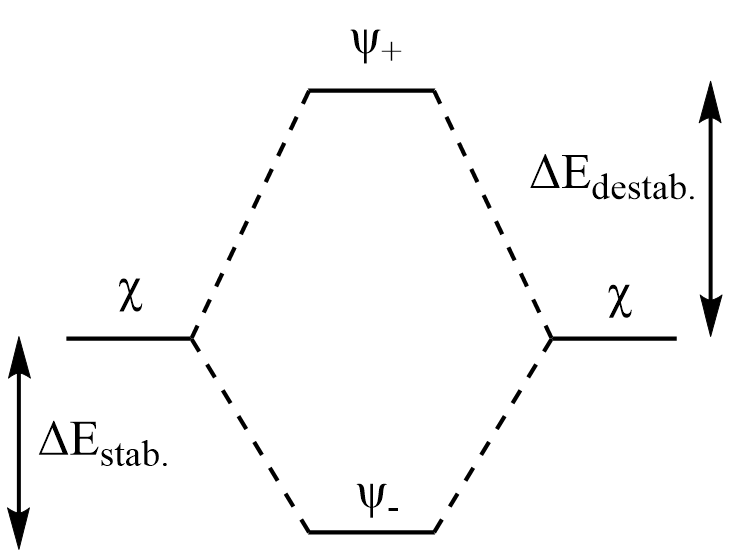
\includegraphics[scale=0.2]{Ch6/energy_profile}
	\caption{energy profile for the interaction of two denegerate orbitals}
	\end{figure}
	
\subsection{Stabilization}

	For two orbitals, ultilizing H\"uckel approximation, the secular determinant becomes:
%
	\[
	\begin{vmatrix}
	\ \alpha_1 - E & \beta       \ \\
	\ \beta        & \alpha_2 - E \ 
	\end{vmatrix} = 
	(\alpha_1 - E)(\alpha_2 - E) - \beta^2 = 0
	\]
%
	Let average energy $\bar{\alpha} = (\alpha_1+\alpha_2)/2$ 
	and energy difference $\Delta = \alpha_2-\alpha_1>0$, then
%
	\[
	E_\pm = \bar{\alpha} \pm \frac{1}{2} \sqrt{\Delta^2 + 4\beta^2}.
	\]
%
	The stabilization energy is:
%
	\[
	\Delta E_{\text{stab}} 
	= \alpha_1 - E_- 
	= -\frac{\Delta}{2} + \frac{1}{2}\sqrt{\Delta^2 + 4\beta^2}
	\]
%	
	Note that here's the failure for Huckel approximation (see \ref{Huckel}): 
	by letting S=0 the stabilization of bonding are equal to the destabilization of antibongding now. \label{sym} \\ \\
%
	Two limiting regimes are important:
%
	\begin{itemize}
	\item If $\Delta = 0$, maximal stabilization equals $|\beta|$.
	\item If $\Delta \gg |\beta|$, expand the square root to the second order:
%	
	\[
	\sqrt{\Delta^2+4\beta^2} = 
	\Delta\sqrt{1+(2\beta/\Delta)^2} \approx 
	\Delta + \frac{2\beta^2}{\Delta}
	\]
%	
	so the stabilization is
%	
	\[
	\Delta E_{stab} = 
	\frac{\left| \langle\chi_1|\hat{H}|\chi_2\rangle \right|^2}{E_2-E_1}
	\]
%	
	which matches second-order perturbation theory, implying:
	\end{itemize}
%
	\[
	\boxed{\text{Smaller energy gaps produce stronger orbital interaction.}}
	\]\label{closer energy}

\subsection{Bond Order and Polarity}\label{polar}

	The bond order is defined as
%
	\[
	b = \frac{1}{2}
	(N_{\text{bonding}} - N_{\text{antibonding}}).
	\]
%
	Larger $b$ implies stronger and shorter bonds.\\ \\
%
	From the coefficient ratio derived from secular equations,
%
	\[
	\frac{c_2}{c_1}
	=
	\frac{\Delta - \sqrt{\Delta^2 + 4\beta^2}}{2\beta},
	\]
%
	we observe:
%
	\begin{itemize}
	\item If $\Delta = 0$, $c_1 = c_2$, nonpolar covalent bond.
	\item If $\Delta > 0$, the lower-energy AO dominates the bonding MO.
	\end{itemize}
%
	Thus:
%
	\[
	\boxed{\text{Molecular orbitals resemble the atomic orbitals closest in energy.}}
	\]
%
	Increasing $\Delta$ shifts electron density toward the lower-energy center, 
	producing bond \emph{polarization}. 
	In the extreme limit, the bond becomes \emph{ionic}.	
	
\section{Conjugate Systems}

\subsection{Linear Conjugate Systems}\label{linear}
	
	For a \emph{linear conjugate system} with $n$ identical orthonormal AOs, all $\alpha$ are equal, 
	only adjacent orbitals have non-zero and equal $\beta$, the secular determinant is:
	%
	\[\begin{vmatrix}
	\ \alpha-E & \beta    &        &          & 		\\
	\ \beta    & \alpha-E & \beta  &          & 		\\
	         & \ddots   & \ddots & \ddots   & 		\\
	         &          & \beta  & \alpha-E & \beta\ \\
			 &			&		 & \beta    & \alpha-E\  
	\end{vmatrix} = 0\]
	%
	With solution:
	%
	\[c_{ij} = \sqrt{\frac{2}{n+1}}\sin\frac{ij\pi}{n+1} \]
	\[E_i = \alpha+2\beta\cos\frac{i\pi}{n+1}\]
	%
	Note that the orbital coefficients resemble the sinusodial wavefunction of 1d potential well, 
	and the energies are like dividing a semicircle into $n+1$ parts as the figure shows.\\ \\
	%
	\begin{figure}[h]
	\centering
	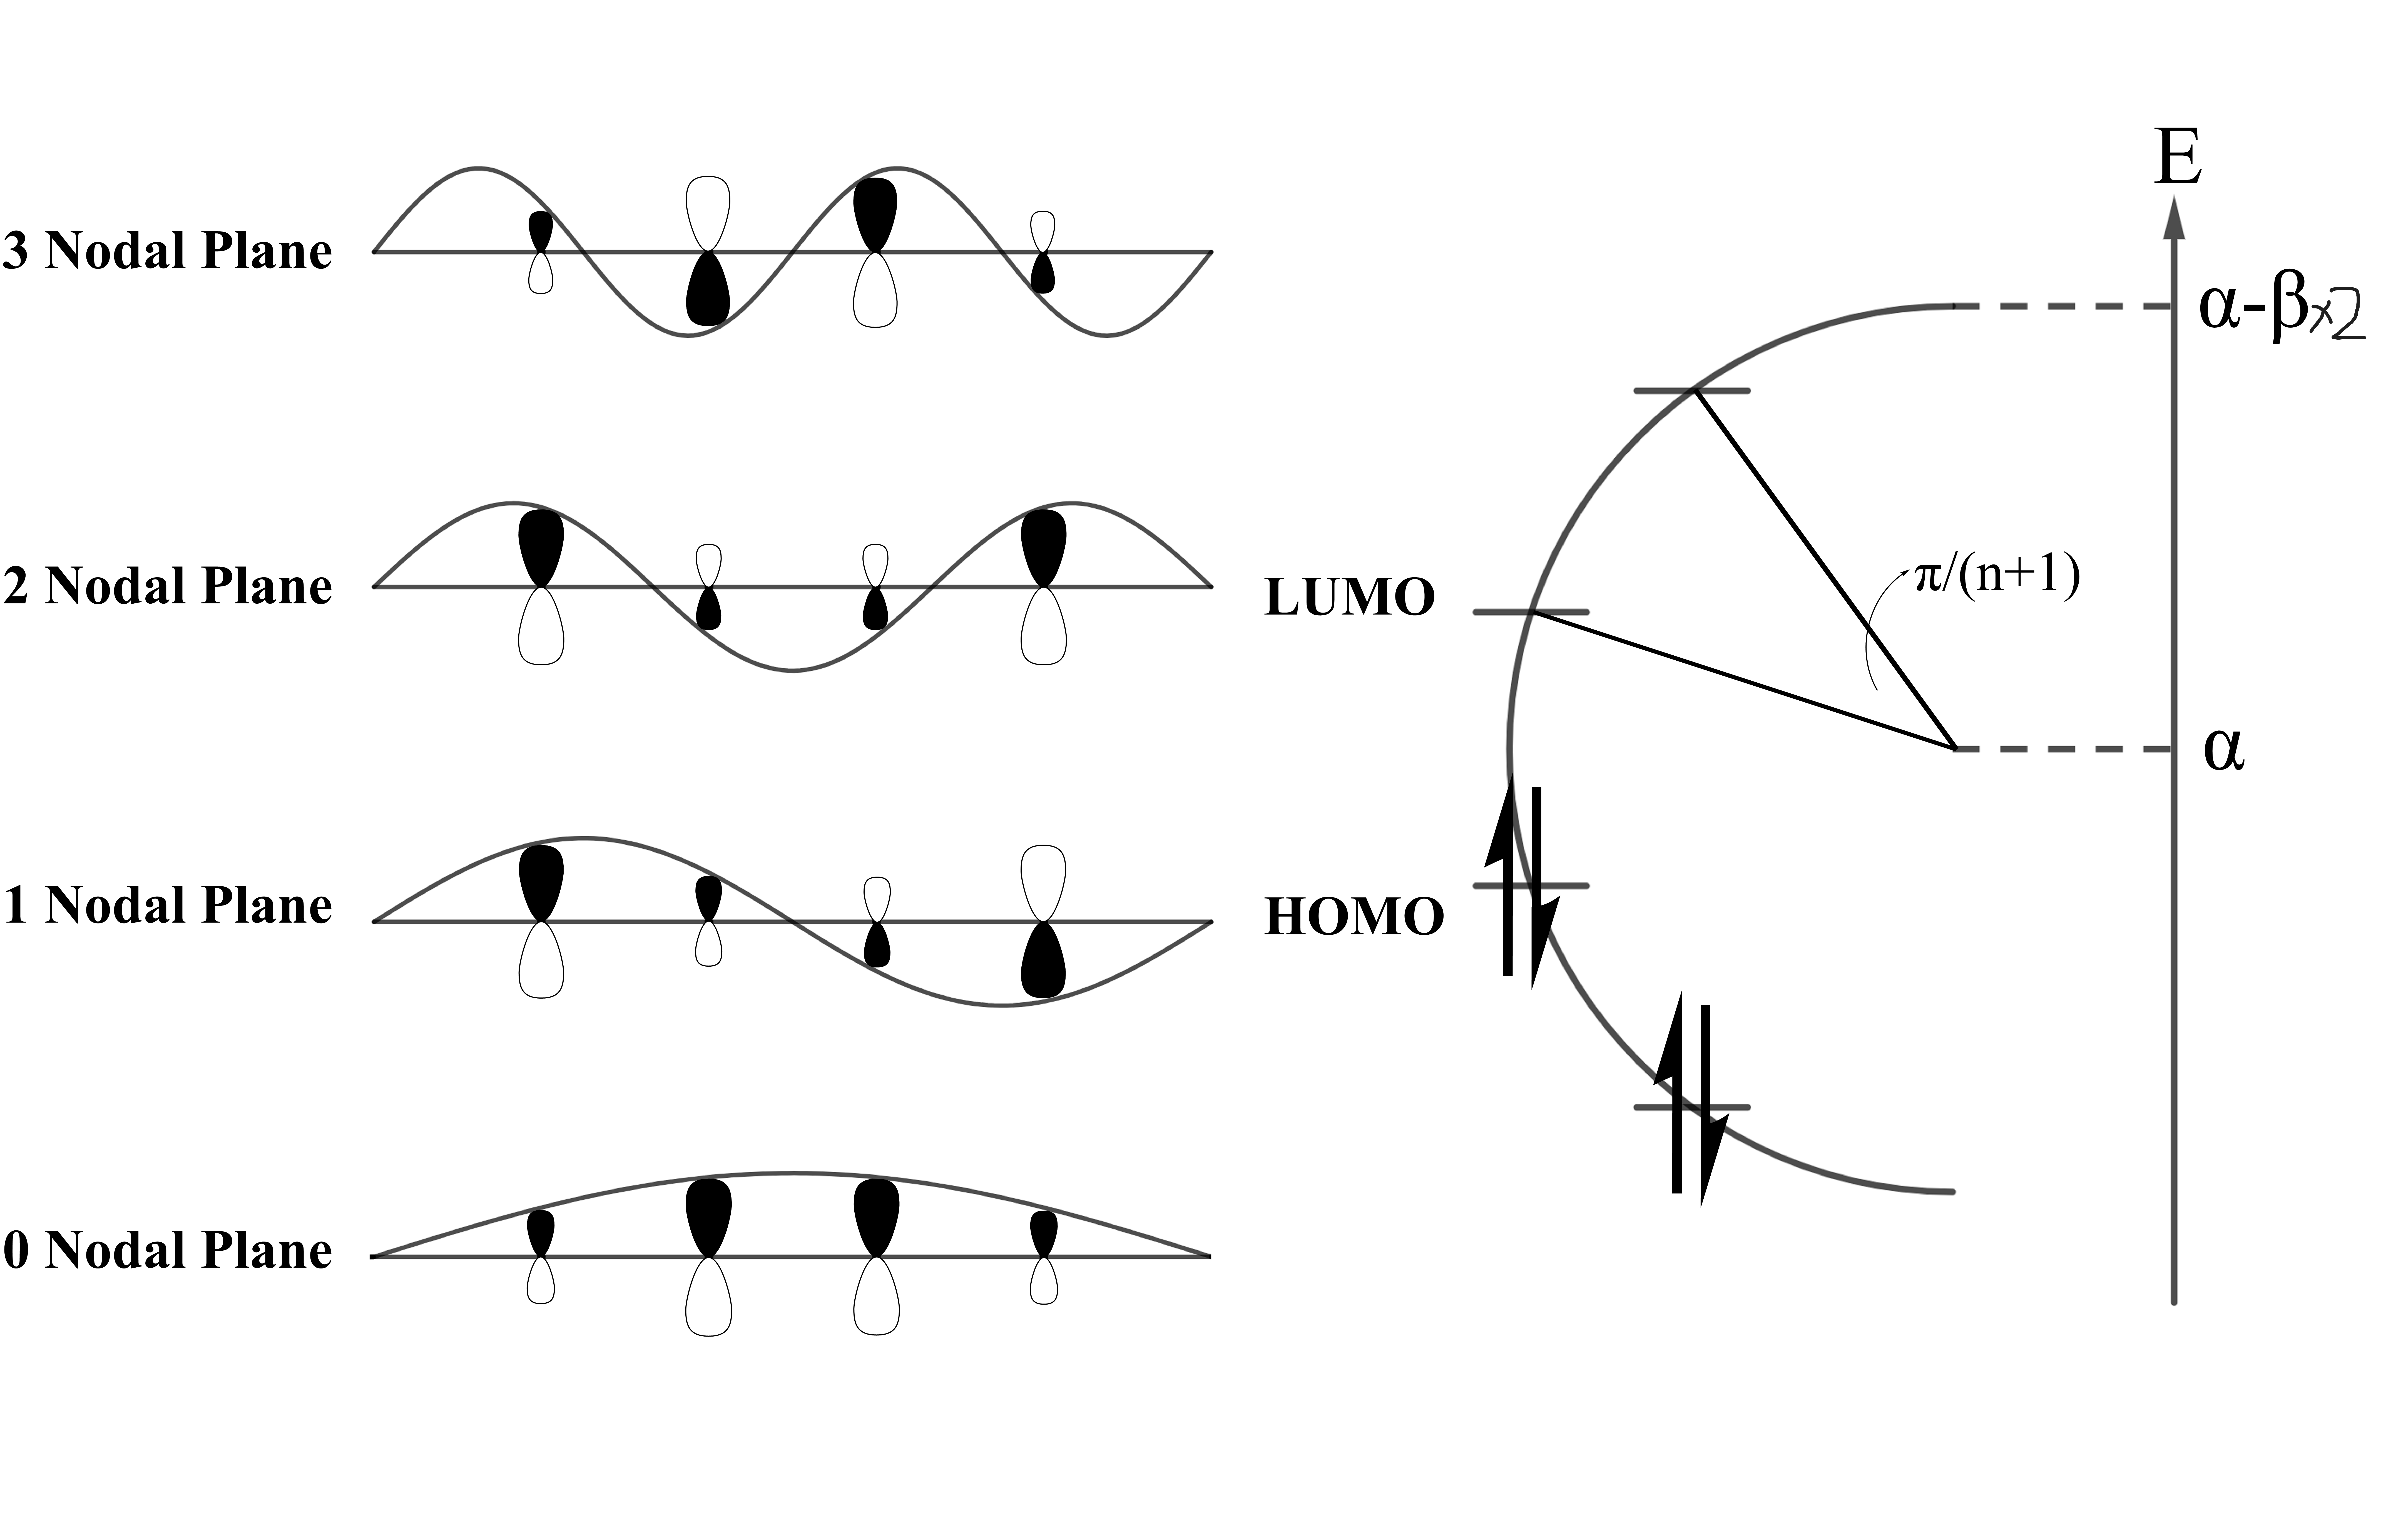
\includegraphics[scale=0.05]{Ch6/conjugation}
	\caption{molecular orbitals of 1,3-butadiene (n=4)}
	\end{figure}
%
	As $n$ increases, the orbital energy can reach lower areas of the circle with lower energy, 
	and their energy is lower than that of $n/2$ ethenes whose energy is $n(\alpha+\beta)$ solved by the same way.
	This stabilization is called \emph{delocalization energy}.\\
	On the other hand, as $n$ increases, $\pi/(n+1)$ decreases, i.e. the \emph{HOMO-LUMO gap narrows} as conjugate system lengthens, 
	leading to a red shift in UV-vis absorption peak.\\ \\
	%
	In the extreme case, as $n$ approaches infinity, the orbitals' energy approaches continuum, becoming an energy \emph{band}. 
	This will be further discussed in \ref{band}.
	
\subsection{Circular Conjugate System: Aromaticity}\label{circonj}

	For a \emph{circular conjugate system}, as it's connected head to tail, the determinant is then:
	%
	\[\begin{vmatrix}
	\ \alpha-E & \beta    &        &          & \beta\	\\
	\ \beta    & \alpha-E & \beta  &          & 		\\
	         & \ddots   & \ddots & \ddots   & 		\\
	         &          & \beta  & \alpha-E & \beta\ \\
	\ \beta	 &			&		 & \beta    & \alpha-E \ 
	\end{vmatrix} = 0\]
	%
	With solution:
	%
	\[c_{ij} =\sqrt{\frac{2}{n}}\sin\frac{2ij\pi}{n}\]
	\[E_i = \alpha+2\beta\cos\frac{2i\pi}{n}\]
	%
	Whose coefficients resemble the wave on a circle, and the energy levels divide the whole circle into $n$ parts.
	Due to the symmetry of circle and the consequent degeneracy, the energy lowers further compared with linear conjugation.\\\ \\
	%
	When $N=4k+2, k\in\mathbb{N}$, all electrons are paired into orbitals below $\alpha$, 
	achieving an extremely stable configuration so called \emph{aromaticity}, however when $N=4k$, 
	two singly occupied orbitals exist, making the molecule less stable, which is called \emph{antiaromaticity}.\\\ \\
	%
	Note that $n$ is the number of AOs and $N$ is the number of electrons. \\\ \\
	%
	Molecular orbitals can also be generated by group theory, see \ref{mo}.
		
	
\section{Molecular Orbital Theory and Valence-Bond Theory}
\subsection{General Molecular Orbital Theory}

	In a molecule, all symmetry-compatible orbitals combine to form $n$ molecular orbitals from $n$ atomic orbitals.
	How to determine whether orbitals are symmetry-compatible is beyond the scope of this chapter, see SALC \ref{salc}.
	Two orbitals interact significantly only if:
%
	\begin{enumerate}
	\item Their symmetries are compatible,
	\item Their overlap integral is nonzero,
	\item Their energies are comparable.	
	\end{enumerate}
%
	By symmetry with respect to the internuclear axis, bonds are classified as:
%
	\begin{itemize}
	\item $\sigma$ bonds: head-to-head overlap, cylindrical symmetry.
	\item $\pi$ bonds: side-by-side overlap, one nodal plane.
	\item $\delta$ bonds: face-to-face overlap, two nodal planes.
	\end{itemize}
%
	\begin{figure}[h]
	\centering
	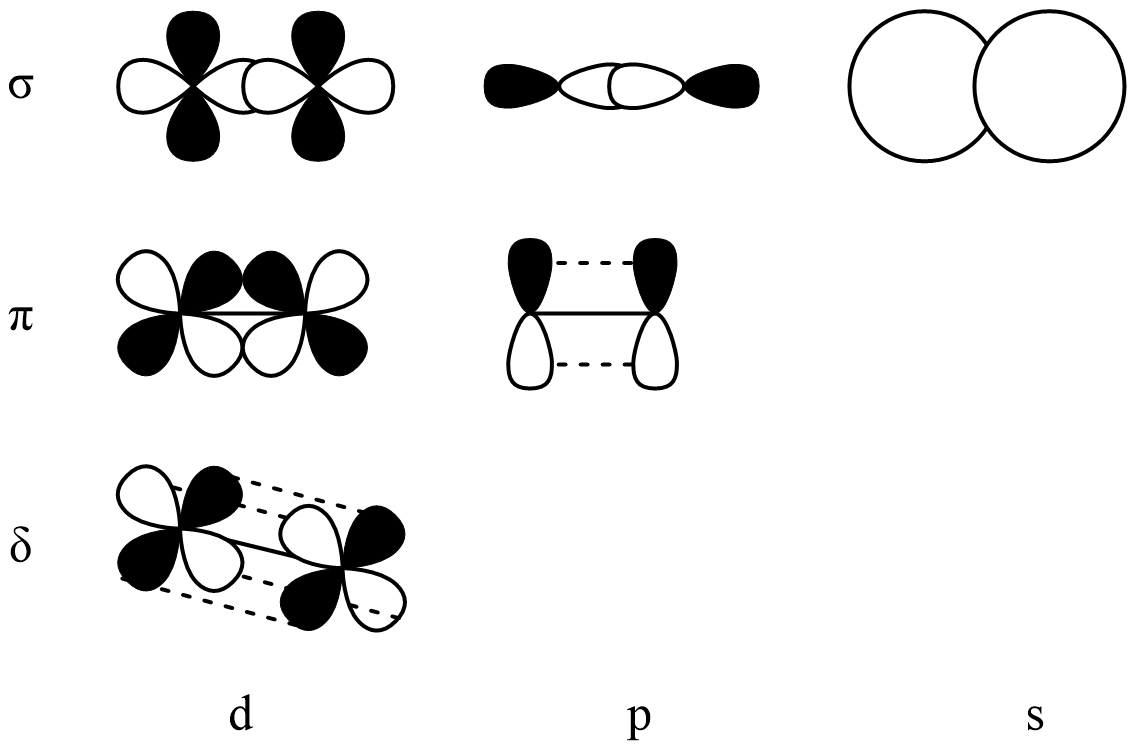
\includegraphics[scale=0.3]{Ch6/VB}
	\caption{three types of covalent bond}
	\end{figure}
%
	Electrons occupy molecular orbitals according to the building-up principle and Pauli exclusion principle (see \ref{pauli}). 
	Bonding characteristics follow directly from orbital occupation and energy ordering.
	
\subsection{Electronic Configuration}

	Consider the case of 2 electrons filling the system of previously discussed ${|\chi_1\rangle, |\chi_2\rangle}$.
	
\subsubsection{Molecular Orbital Theory}

	In MO theory, the two orbitals first combine and then electrons fill in.\\ \\
%	
	The ground state is two electrons filling $|\psi_-\rangle$ with their spins paired.
	Combining the spacial state and spin state and we can form the unnormalized Slater determinant (see \ref{slater det}) of this system.
%	
	\[
	\psi = 
	\underbrace{\psi_-(1)\psi_-(2)}_{\text{spacial part}}
	\underbrace{[\alpha(1)\beta(2) - \alpha(2)\beta(1)]}_{\text{spin part}} = 
	\begin{vmatrix} 
	\ \psi_-\alpha(1) & \psi_-\beta(1)\ \\ 
	\ \psi_-\alpha(2) & \psi_-\beta(2)\ 
	\end{vmatrix}
	\]
%	
	Two excited states can also be generated in the same way.\\ \\
%	
	The two singlet states can then form an orbital basis and undergo the secular process again to get a more accurate result.
	
\subsubsection{Valence-Bond Theory}

	In valence-bond theory, every electron is considered to reside on one atomic orbital.
	For a system with 2 orbitals and 2 electrons, there're two ways to place the electrons:
%	
	\[
	\psi_1 = \chi_1(1)\chi_2(2)
	\qquad
	\psi_2 = \chi_1(2)\chi_2(1)
	\]
%	
	Use these two states as the set of basis functions and solve the secular equation gives:
%	
	\[
	\psi_- = \frac{\psi_1+\psi_2}{\sqrt{2+2S^2}} 
	\qquad 
	\psi_+ = \frac{\psi_1-\psi_2}{\sqrt{2-2S^2}}
	\]
%	
	where $S$ is the overlap of ${|\chi_1\rangle, |\chi_2\rangle}$ but not $\psi_1$ and $\psi_2$.\\ \\
%
	Similar to molecular orbital theory, valence-bond theory also gives bonding and antibonding orbitals, 
	and actually this theory is developed earlier.\\ \\
%	
	The VB theory and MO theory are identical and both correct as an interpreting theory. 
	VB theory fills in electrons first then combines the orbitals while MO theory combines orbitals first then fills in electrons.\\
	However, in case of \emph{hypervalent compounds}, valence shell orbitals aren't adequate for forming so much bonds, 
	so VB theory has to treat them as \emph{zwitterions} or (once popular but turned out to be wrong) take advantage of orbitals from outer shells,
	while MO theory are more skilled at handling such problems with symmetry. See \ref{salc}.
	
\subsection{Hybridization}

	When more than one bond is needed to be formed around a central atom, 
	most likely would it like to adopt a configuration with the highest symmetry in order to increase degeneracy and lower the overall energy.
	However the orientation of atomic orbitals is fixed, 
	so the orbitals with energy close to one another would recombine linearly to match the symmetry, see \ref{hybridization} for details.\\\ \\
	%
	As said, orbitals whose energy are closer have a better effect of hybridization (see \ref{closer energy}) 
	so lighter atoms tend to hybridize but heavier atoms do not, because the energy gap between adjacent subshells widen as period number increases, 
	which is especially significant to the main group $sp^n$ hybridization 
	due to $d,f$ block insertion and the consequent $6s^2$ inert pair effect (see \ref{radius}).
	Aside from that, subgroup elements do not take their outermost $d$ electrons into hybridization 
	but main group elements do, and almost always, hybridize their valence shell $s,p$ electrons.
	
\subsection{Bent's Rule and $sp^n$ Hybridization}

	Because the $s$ orbital has lower energy and smaller radius than the $p$ orbitals in the same shell, 
	it experiences more nuclear charge and thus becomes more electronegative. 
	Therefore atoms, whose hybridized orbital have more $s$ component, are more electronegative and more stable to lone pairs, 
	which also implies less basicity, 
	and positive charges or empty orbitals tend to choose ones with more $p$ component to let electrons occupy the orbitals with more $s$ character.
	The angle $\theta$ between hybridized orbitals are given by:
	\[\cos\theta = -\frac{n_s}{n_p}\]
	%
	\emph{Bent's Rule} qualitively describes the effect of substituents on hybridization:\\\ \\
	For an \emph{electron withdrawing group}, the electron cloud of the bond will shift towards the substituent, 
	lowering the electron density of the atomic orbital of the central atom 
	while an \emph{electron donating group} does the opposite and increase the electron density.
	And in order to achieve the lowest overall energy, 
	orbitals with higher energy tend to form a bond with lower electron density (less populated), 
	and orbitals with lower energy want to be populated with more electron density.\\\ \\
	Therefore, bonds to an EWG have more $p$ component and bonds to an EDG have more $s$ component.
	In the extreme case, as discussed earlier, are the vacant orbitals and lone pairs.
	
\section{Bonding in Clusters}
\subsection{Single Polyhedra}
When fragments that already have its bonding structure but lack electrons, 
they tend to polymerize into clusters using their empty or singly occupied orbitals. 
These electron-deficient clusters have to invoke multi-center bonds to alleviate electron shortage.
For a cluster like this, we treat the bonding paradigm as fully delocalized orbitals around a imaginary geometrical center, 
for counting all the 3c-2e bonds would be annoying.\\ \\
%
Then the orbital contribution of each vertex fragment can be separate into two orthogonal irreps according to local symmetry, 
namely radial and tangential. (For irreps, see \ref{irrep})
\begin{itemize}
\item Radial orbitals point towards the center, thus along the principal axis: $A_1$ irrep must be assigned subject to the local vertex symmetry.
\item Tangential orbitals tangent to the circumscribed sphere: Spans a 2 dimensional tangent plane, $E$ irrep assigned subject to local symmetry.
\end{itemize}
%
Therefore each fragment should contribute 1+2 orbitals to the polyhedral skeleton, and hence overall $3n$ orbitals.
These orbitals are usually the highest in energy and are empty or singly occupied, and thus:
\begin{itemize}
\item Main group fragments: 4 orbitals. One lone pair or existing bond should be excluded (-2e).
\item Transition metals: 9 orbitals. 6 orbitals with 12 electrons should be excluded (-12e).
\end{itemize}
Note that if a main group element is enclosed inside the cluster, often seen if there's only a single C or P without H attaching to them, 
their `lone pair' needn't be subtracted.
First consider radial orbitals: all bonds can overlap because they all point at a same point. 
Employing H\"uckel approximation (see \ref{Huckel}): $\alpha^r,\ \beta^r<0$ same for all orbitals, then the matrix element for Hamiltonian is:
\[\mathbf{H}_{ij}^r = \alpha^r \delta_{ij} + \beta^r (1-\delta_{ij})\]
Which corresponds to a matrix with $\alpha^r$ in the diagonal line and others all $\beta^r$, thus:
\[\mathbf{H}^r = (\alpha^r - \beta^r)\mathbf{I} + \beta^r\mathbf{J}\]
where J is the matrix of ones with rank 1, mapping all vectors onto line defined by $\mathbf{v}=(1,1,1...)^{T}$.\\
Therefore it has $n$ orthonormal eigenvectors: 
one on the line, corresponding eigenvalue $n$, and other $n-1$ span the plane perpendicular to the line with eigenvalue 0.\\
The spectrum of $\mathbf{H}^r$ is then:
\begin{align*}
& \text{Singly degenerate}\quad\ \ \ E=\alpha^r + (n-1) \beta^r < \alpha^r & \text{ strong bonding}\\
& n-1 \text{ fold degenerate}\ \ E = \alpha^r - \beta^r > \alpha^r  & \text{ antibonding}
\end{align*}
The consider tangential orbitals: only adjacent orbitals overlap.
This is the 3 dimensional version of cyclic conjugation (see \ref{circonj}) whose Hamiltonian has spectrum symmetric about $\alpha^t$.
Hence among total $2n$ tangential orbitals, 
half are bonding orbitals that have energies lower than $\alpha^t$,
and the other half have energies above $\alpha^t$.
\[\boxed{\text{ Total orbital count: } n+1 \text{ bonding and } 2n-1 \text{ antibonding }}\]
Therefore $n$ vertex fragments with $(n+1)$ skeletal electron pairs will form closed deltahedral clusters, denoted as \emph{closo}
For those skeletal electron pairs more than $(n+1)$, we can
\begin{itemize}
\item Consider having imaginary 3-orbital 2-eletron fragments so that they form \emph{closo} deltahedra and then take those vertices away;
\item Or, \emph{in electron precise clusters}, one more pair of electrons will fill one antibonding orbital, locally break one edge will do.
\end{itemize}
we name those geometrical configurations with more than $(n+1)$ electrons in table \ref{table10.1}\\ \\
Take $\rm Co_3(CO)_9CH$ as an example: 
\[\text{SEP} = \frac{1}{2}(3\cdot9+9\cdot2-3\cdot12+1\cdot3)=6\quad\Rightarrow\quad \text{SEP}=n+2\]
Therefore, the structure should be \emph{nido}-trigonal bipyramid, should it?
There's a coincidence here, limited to tetrahedra, that when SEP=6, it matches the electrons pair needed for 6 tetrahedral localized bonds.
Thus $\rm Co_3(CO)_9CH$ but not a butterfly-shape as in \emph{nido}-trigonal bipyramid.\\ \\
This exception that \emph{$n=4$, SEP=6 may corresponds to tetrahedron} is common in metal clusters 
as this form of bonding often matches better with octahedral coordination environment.
\begin{figure}[h]
\centering
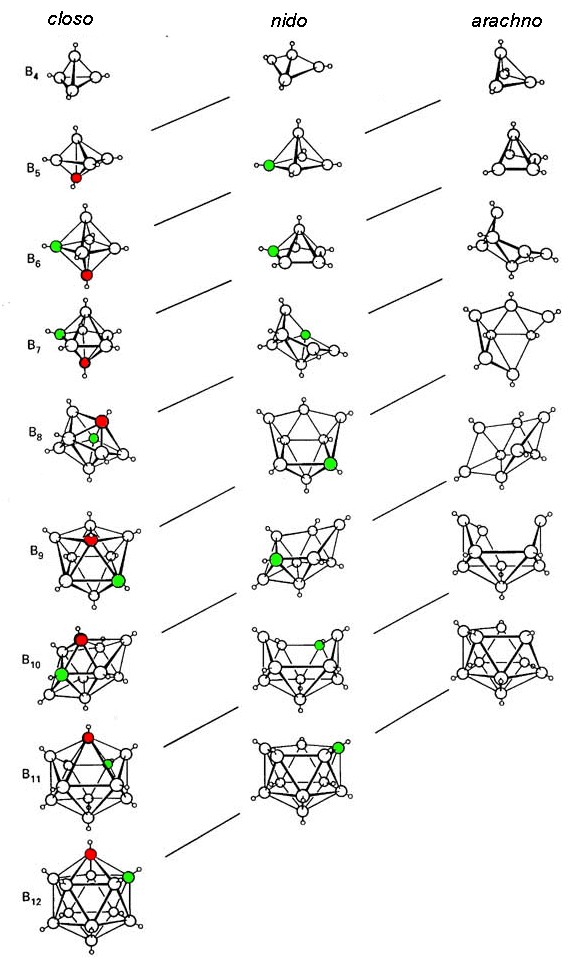
\includegraphics[scale=1]{Ch6/wadesrule}
\caption{Graphic Description of PSEPT Deltahedra}
\end{figure}
\begin{table}
\centering
\begin{tabular}{|cl||cl|}
\hline
Vertices&Name&Vertices&Name\\
\hline
4&Tetrahedron&9&Triaugmented Trigonal Prism\\
5&Trigonal Bipyramid&10&Biaugmented Square Antiprism\\
6&Octahedron&11&Edge-Contracted Icosahedron\\
7&Pentagonal Bipyramid&12&Icosahedron\\
8&Snub Disphenoid&&\\
\hline
\end{tabular}
\caption{Names of Deltahedra}\ \\
\begin{tabular}{@{}cl@{}}
\toprule
\ SEP&Configuration\ \\
\midrule
\ $n+1$&\emph{closo}\\
\ $n+2$&\emph{nido}\\
\ $n+3$&\emph{arachno}\\
\ $n+4$&\emph{hypho}\\
\bottomrule
\end{tabular}
\caption{Polyhedra Types in PSEPT}
\label{table10.1}
\end{table}
\subsection{Condensed Polyhedra}
If SEP $\leq n+1$, implying the cluster is still electron-deficient, polyhedra must condense to meet their need for electrons.
What we're really concerned about is the bonding on the condensing boundary, 
so localized valence-bond theory is much more handy than molecular orbitals.\\ \\
Assume the shared region consists of $k$ vertices and $m$ edges, 
and in terms of valence-bond, that's $k$ atoms with $3k$ orbitals and $m$ bonds.
Forming $m$ bonds need $2m$ orbitals but only the $m$ bonding orbitals to SEP, 
and the number of lone pairs is then $3k-2m$ which is also taken into SEP count.\\
Therefore the total SEP shared is:
\[(3k-2m)+m=3k-m\ \text{SEPs shared}\]
These SEPs are counted twice in isolated polyhedra, so in the condensed case they need to be subtracted.
And now, for $n$ vertices with SEP shortage, we can utilize this method to break them into two separate polyhedra and then condense them, 
referring to table \ref{condense}.\\ \\
\begin{table}
\centering
\begin{tabular}{|*6{c|}}
\hline
Sharing: & Vertex & Edge & Triangular Face & Tetragonal Face & Tetragonal Face  \\
\hline
Vertices Add to $n$ & 1 & 2 & 3 & 4 & 4\\
$(3k-m)$ Add to SEP& 3 & 5 & 6 & 7 (With Diagonal) & 8\\
\hline
\end{tabular}
\caption{Shared Part of Condensed Polyhedra}
\label{condense}
\end{table}
An important example is that, for augmenting a triangular face, we can treat it as sharing a triangular face with a tetrahedron.
And, as a localized tetrahedron has SEP=6, \emph{capping with a localized tetrahedron cause no change in SEP}.\\ \\
Take $\rm B_{20}H_{16}$ as an example:
\[\text{SEP} = \frac{1}{2}(20\cdot3+16\cdot1-20\cdot2)=18=n-2\]
Then it must be a condensed polyhedra. After trying, we found that sharing a tetragonal face without diagonal gives:\\
\[n=20+4=24,\ \text{ SEP}=18+8=26\quad\Rightarrow\quad\text{Two \emph{closo}-Icosahedra}\]
Which matches the experimental result.
\subsection{Isolobal Principal}
As each vertex fragment contributes only 3 orbitals to the cluster, the pattern of filling these skeletal orbitals are finite.
Fragments with the same electronic configuration in the 3 skeletal orbitals are \emph{isolobal}, and they form similar clusters.\\
For example, the number of skeletal electrons of $\rm Co(CO)_3$ is $9+2\cdot3-12=3$, which is isolobal to a $\rm CH$ fragment;
a $\rm CH$ with 3 skeletal electrons are isolobal with a $\rm BH^-$ fragment, so we anticipate 
$\rm Co_3(CO)_9CH$ having the same structure as $\rm C_4H_4$ and $\rm B_{10}C_2H_{12}$ having the same structure with $\rm [B_{12}H_{12}]^{2-}$, and that is the case.
	
	 
	
	
	
	
	
	
	
	